This section presents the hardware behind \textit{Hydrotracker}.  Below, we outline the materials used, the sensing principles, the mechanical base design and the full setup procedure.

\subsection{Materials Used}
The following materials were used in constructing a functional prototype of our system:
\begin{itemize}
\item \textbf{Arduino Uno board} – the central microcontroller used to read sensor data and handle communication logic.
\item \textbf{RFM22 ISM Transceiver module} – enables wireless communication between each coaster and a central receiver node.
\item \textbf{3kg Load Cell} – senses the weight of the glass placed on the coaster.
\item \textbf{HX711 Amplifier Module} – amplifies and digitizes the low-voltage analog signal from the load cell.
\item \textbf{3D-printed coaster base} – a custom mechanical housing for the sensor and load distribution.
\item \textbf{LED + 470 $\Omega $ resistor} – provides visual feedback for the taring process.
\item \textbf{Push button} – used to initiate the taring routine manually.
\end{itemize}
For the calibration procedure, we also used:
\begin{itemize}
\item A standard empty water glass.
\item A digital kitchen scale (±1 g precision).
\end{itemize}

\subsection{Load Cell}
The core of the system’s sensing capability lies in the load cell. A load cell is a transducer that converts the force (weight) applied to it into an electrical signal. When an object is placed on the load cell, it slightly deforms (Fig~\ref{fig:loadcell_deforms}). This deformation changes the electrical resistance inside the sensor (Fig~\ref{fig:loadcell-circuit-comparison}), which is then converted into a voltage signal proportional to the weight. This signal can be read by a microcontroller (e.g., Arduino) to determine how much the object weighs, up to a maximum of 3kg. In our case, the 3kg bar-type load cell is placed beneath a flat surface where the glass rests (Fig: \ref{fig:cup-base-views}) .

Since the voltage output from a load cell is very low (typically in the mV range), we use the HX711 module — a high-resolution 24-bit ADC amplifier — to digitize this signal and make it readable by the Arduino (Fig:~\ref{fig:system-setup-views}).
\begin{figure}[H]
    \centering
    \begin{subfigure}[b]{0.45\linewidth}
        \centering
        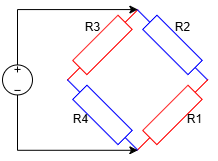
\includegraphics[width=\linewidth]{load cell images/loadcell_curcuit-.drawio.png}
        \caption{Load cell circuit without weight}
        \label{fig:loadcell-weight}
    \end{subfigure}
    \hfill
    \begin{subfigure}[b]{0.45\linewidth}
        \centering
        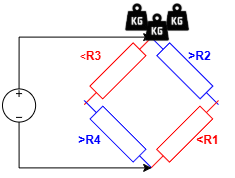
\includegraphics[width=\linewidth]{load cell images/loadcell_curcuit-weight.drawio.png}
        \caption{Load cell circuit with weight}
        \label{fig:loadcell-noweight}
    \end{subfigure}
    \caption{Comparison of load cell circuit states: with and without applied weight}
    \label{fig:loadcell-circuit-comparison}
\end{figure}
\begin{figure}[H]
    \centering
    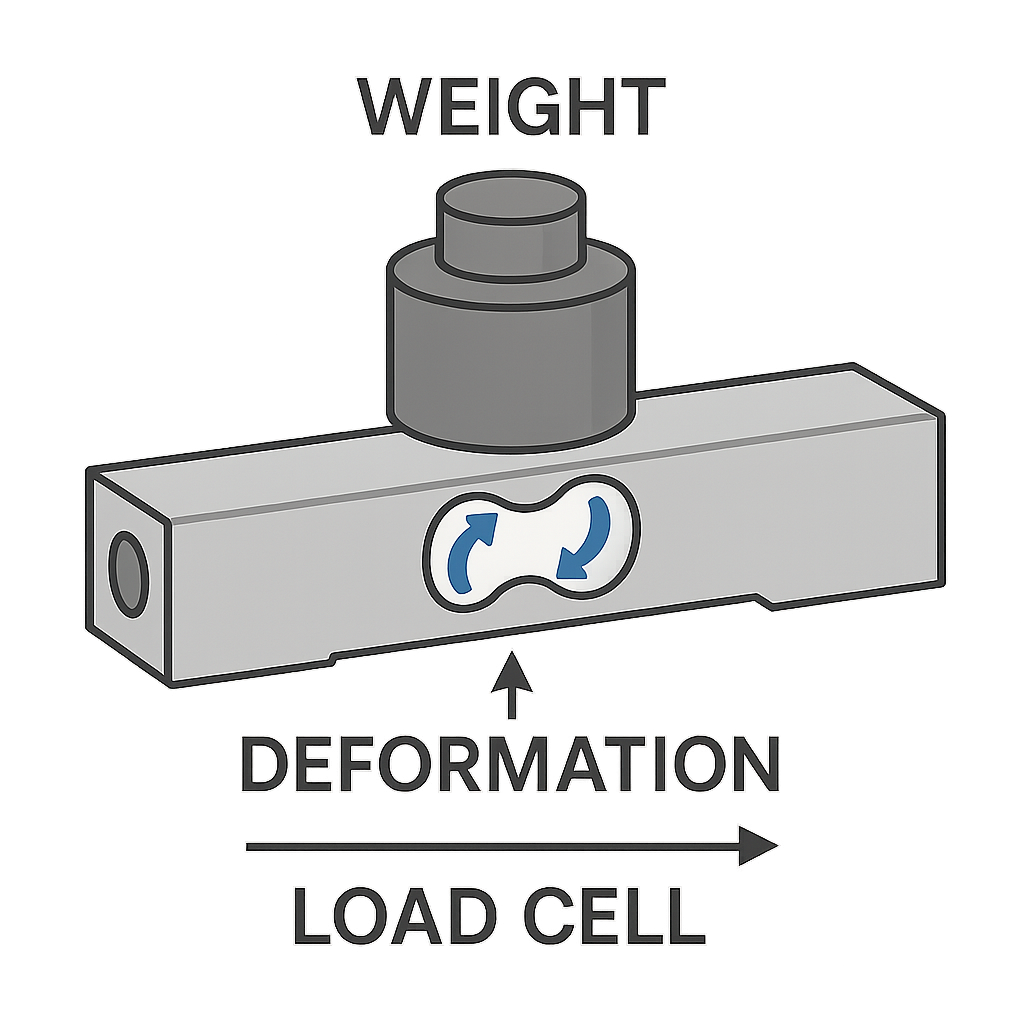
\includegraphics[width=0.35\linewidth]{load cell images/load cell deformation no back.png}
    \caption{Load cell slightly deformates when weight is placed on it}
    \label{fig:loadcell_deforms}
\end{figure}

\subsection{LED-Resistor-Button}
A small but essential subsystem in our design is composed of a push-button, an LED, and a 470 $\Omega$ resistor. This circuit provides user interaction and visual feedback during the taring process of the load cell.

When the system is powered on or reset, the load cell may carry residual mechanical offsets — due to the coaster’s base structure or the inherent weight of an empty cup. To correct this, we implement a manual taring mechanism, initiated by the user via the button.
The button is connected to a digital input pin on the Arduino. When pressed, it triggers the execution of a tare function. This function sets the current output of the HX711 as the new zero reference, assuming the only weight applied is that of the empty cup.

To indicate the progress of this operation, an \textit{LED} is also included. It is connected in series with a 470 $\Omega$ resistor to limit current and is wired to another digital pin configured as an output. When taring is in progress, the LED turns on. Once the process is complete, the LED switches off, notifying the user that the system is ready for use.

\subsection{3D printed cup base}
The physical housing of the coaster is critical to ensure consistent force transfer from the glass to the sensor. Our design consists of two %interlocking 
3D-printed shells (top and bottom). The upper platform is where the base of the glass rests, designed to %evenly distribute the load
concentrate the load to the edge of the load cell for maximum accuracy.
This geometry ensures that vertical force is transmitted directly through the center of the load cell, minimizing measurement noise due to tilting or off-center loading. Figures \ref{fig:base-bottom} and \ref{fig:base-side} show a bottom and a side view of the base design, with the load cell integrated.

\begin{figure}[H]
    \centering
    \begin{subfigure}[b]{0.45\linewidth}
        \centering
        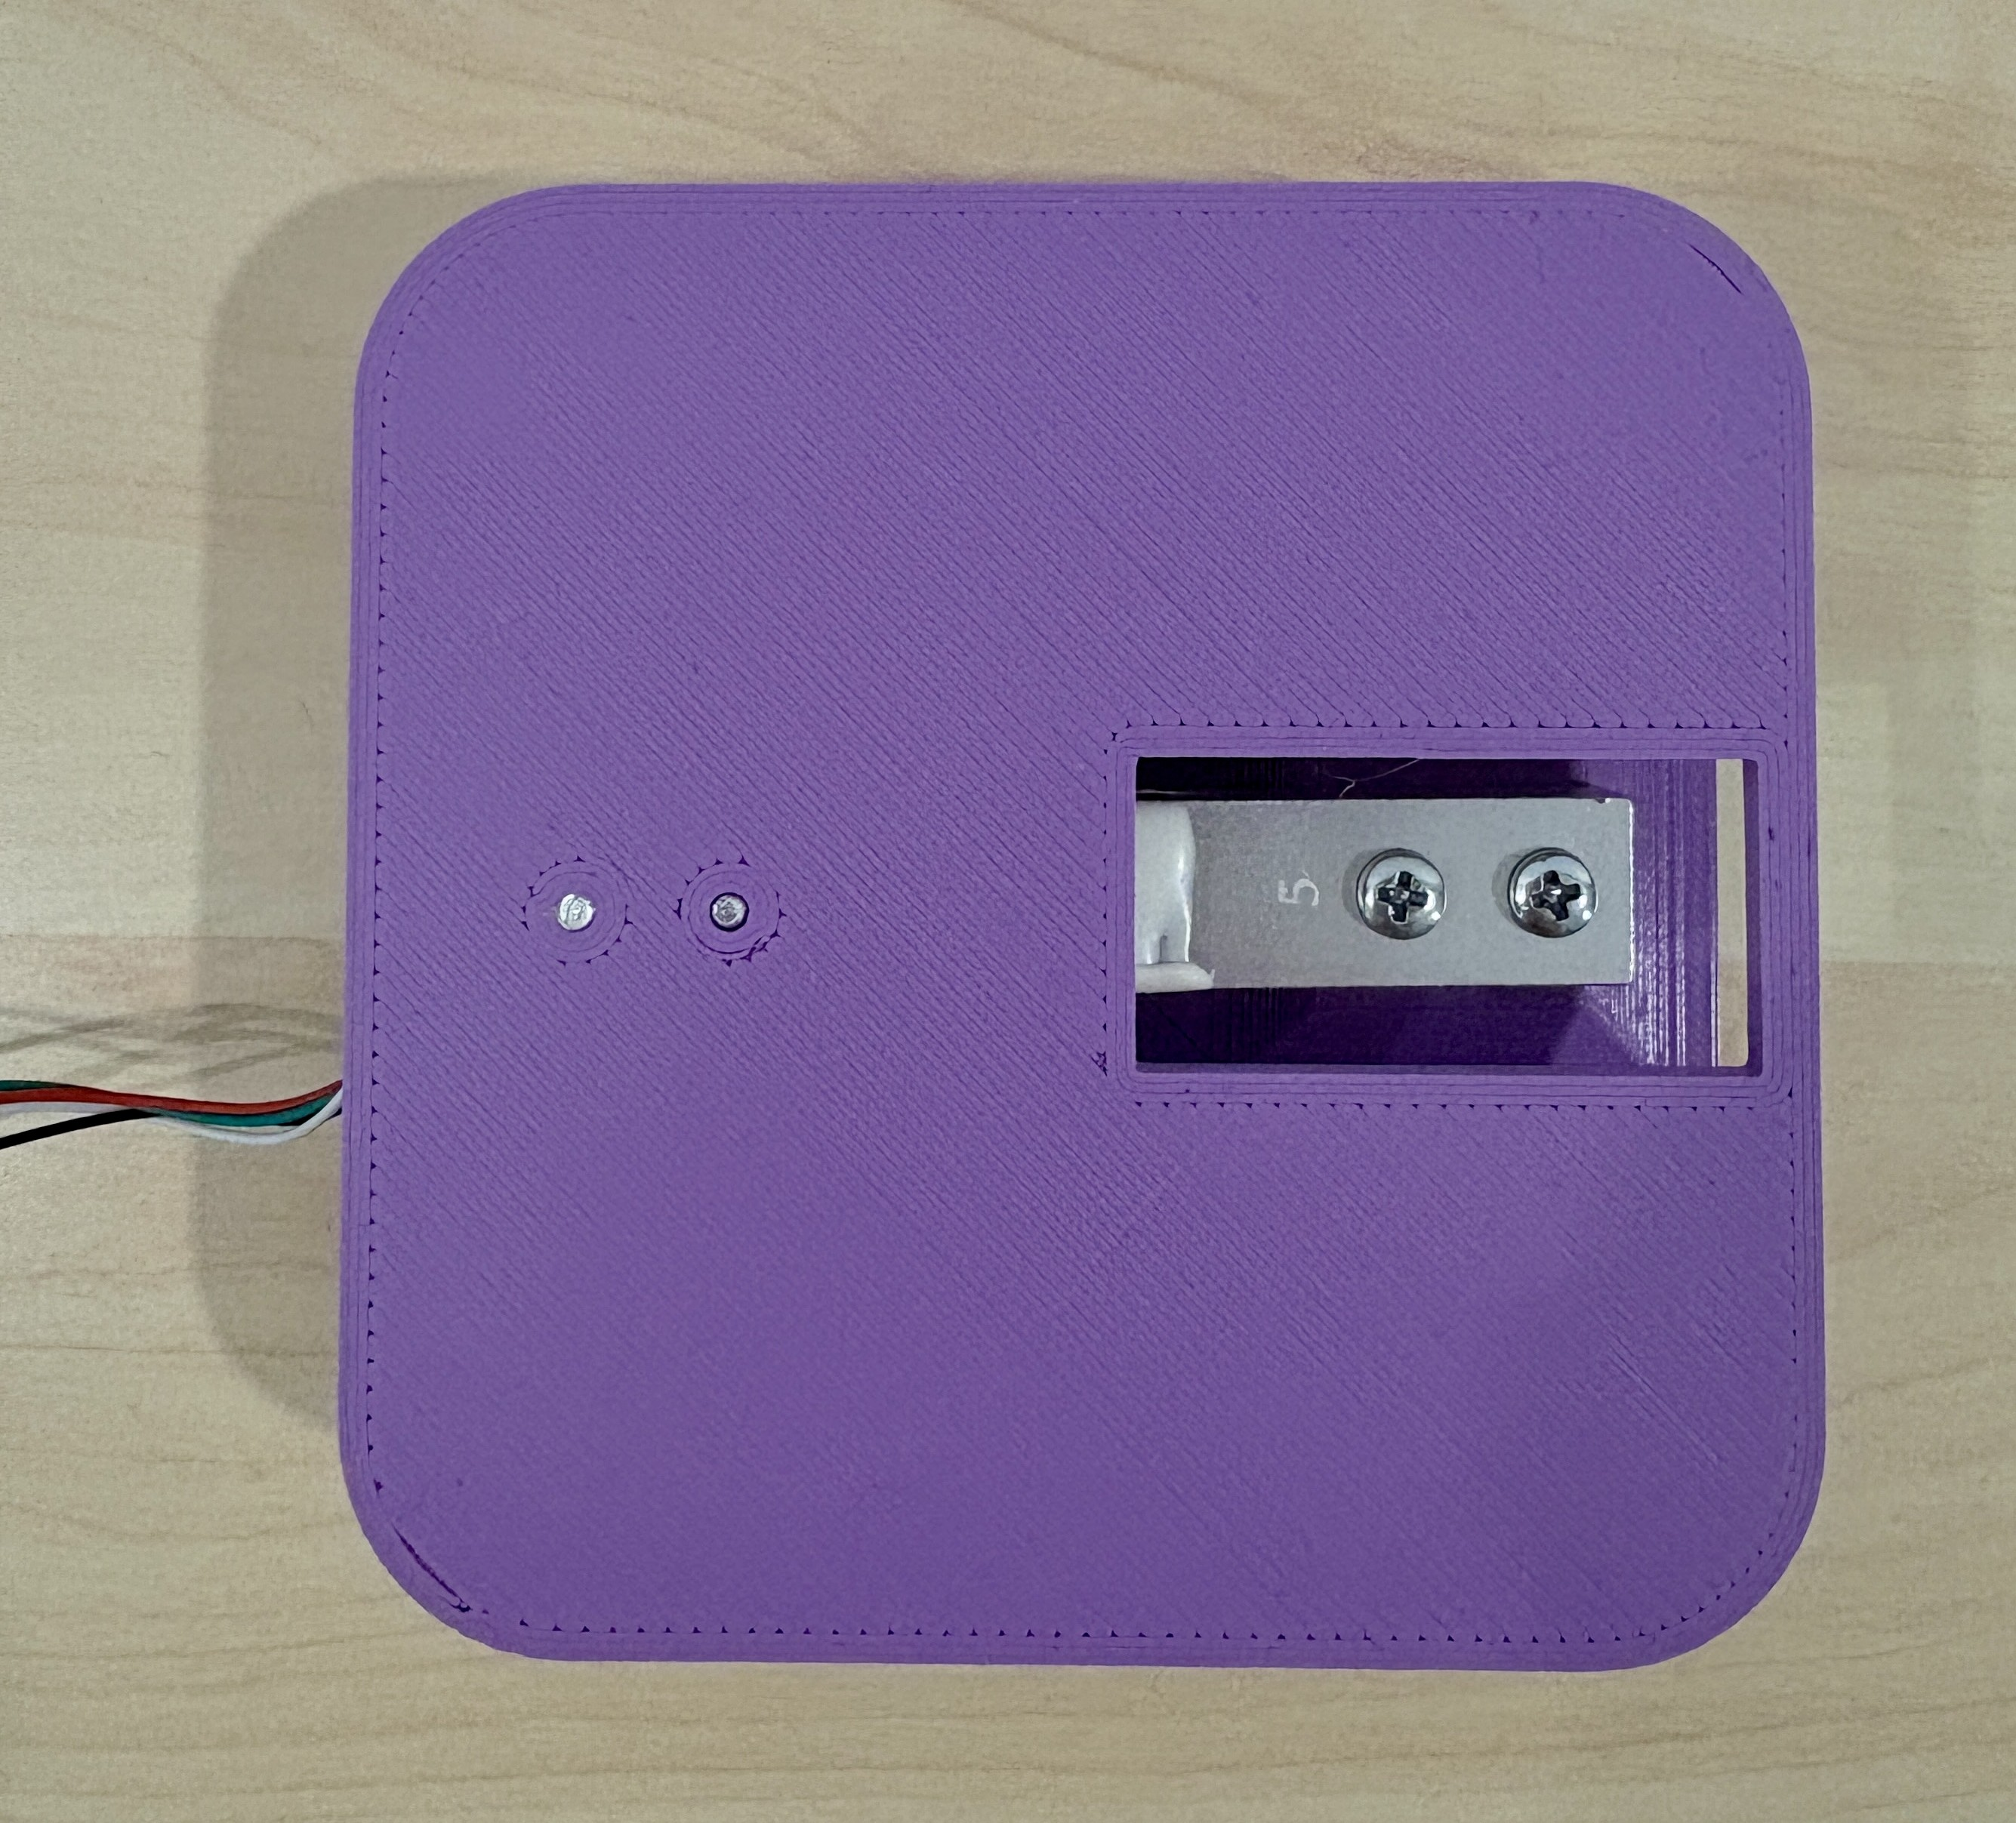
\includegraphics[width=\linewidth]{setup_images/base-bottom-view.jpg}
        \caption{Bottom view of the cup base}
        \label{fig:base-bottom}
    \end{subfigure}
    \hfill
    \begin{subfigure}[b]{0.45\linewidth}
        \centering
        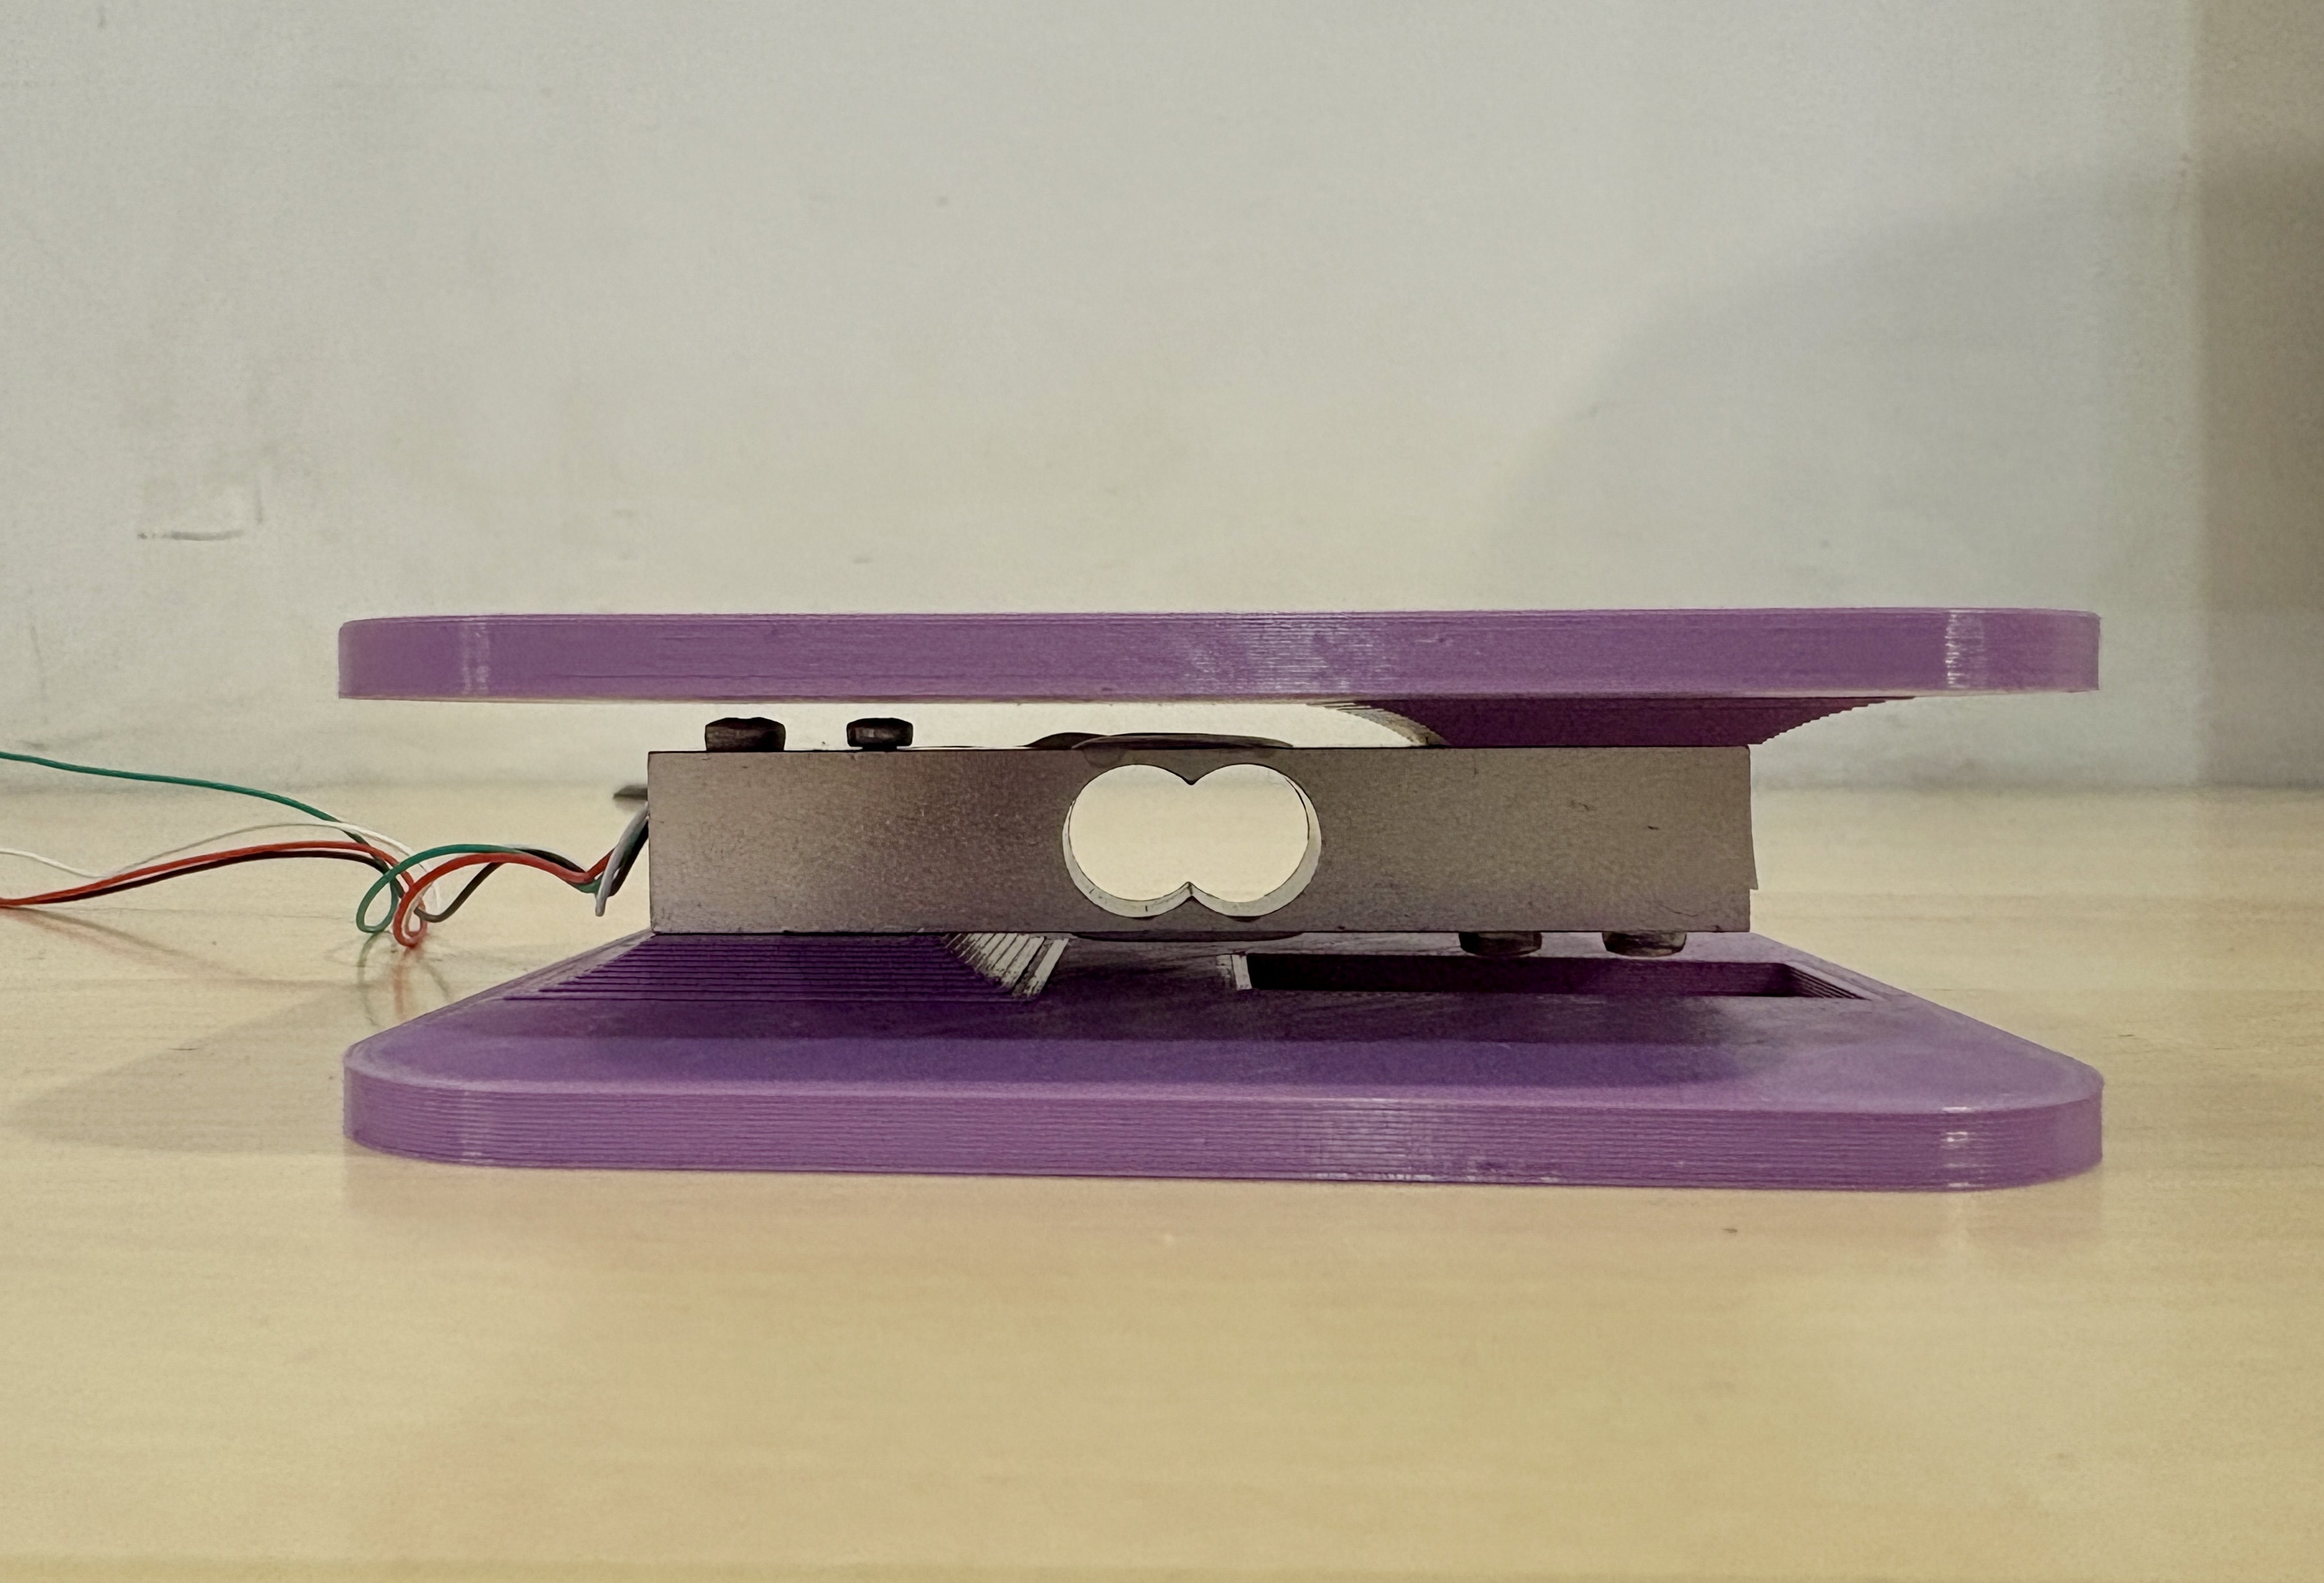
\includegraphics[width=\linewidth]{setup_images/base-side-view.jpg}
        \caption{Side view of the cup base}
        \label{fig:base-side}
    \end{subfigure}
    \caption{3D-printed coaster base: structural views}
    \label{fig:cup-base-views}
\end{figure}

\subsection{Set-up}
The system setup consists of four primary components working together: the mechanical base, the sensing subsystem, the user interface circuit, and the wireless communication module.

The load cell is mounted securely within the custom-designed 3D-printed base. Its output is routed to the HX711 amplifier module, which is responsible for digitizing the analog signal. The HX711 is then connected to the Arduino Uno, allowing the microcontroller to receive precise weight data.

\begin{figure}[H]
    \centering
    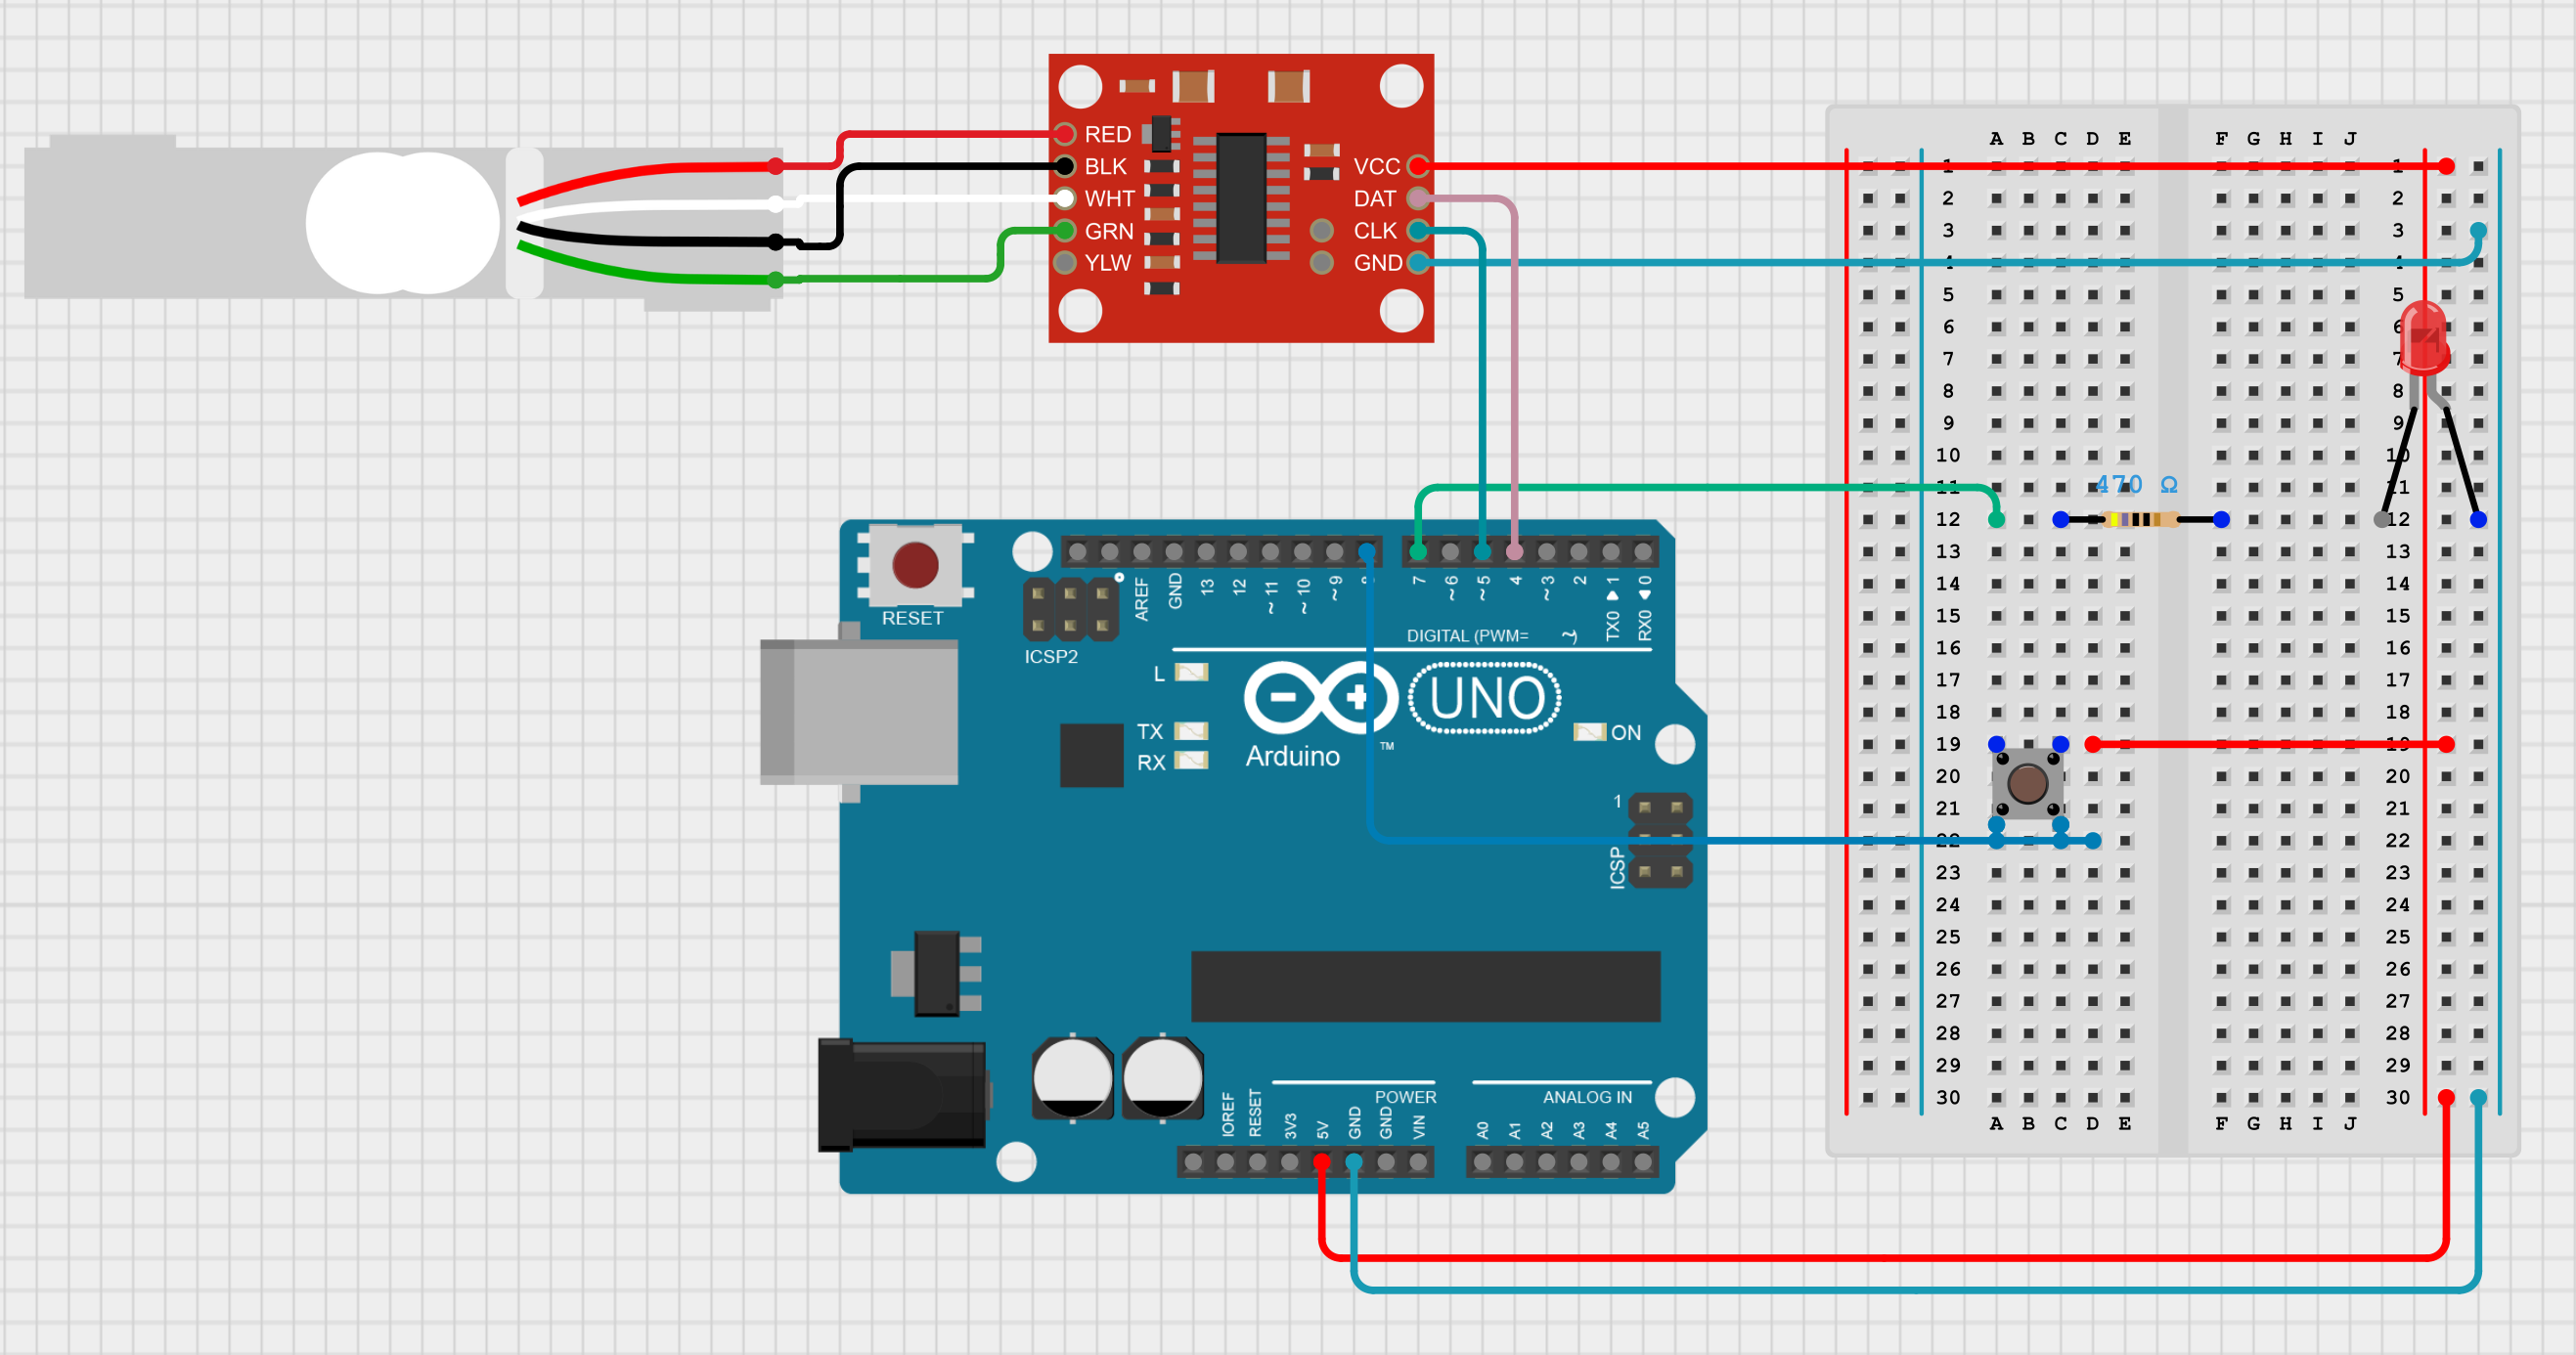
\includegraphics[width=\linewidth]{load cell images/circuit.png}
    \caption{System connection diagram}
    \label{fig:circuit}
\end{figure}

On the breadboard, the push-button and LED are in series with the 470 $\Omega$ resistor. The button is connected to a digital input pin and is used to trigger the taring process, while the LED is connected to an output pin and provides visual feedback indicating the system’s readiness.

To enable communication between multiple coaster nodes and a central monitoring station, the system incorporates an RFM22 wireless transceiver, connected to the Arduino via SPI. This module transmits each node’s state information (\texttt{EMPTY}, \texttt{NOTEMPTY}, \texttt{NOTEXIST}) to a receiver, which updates the graphical user interface accordingly.

The full connection diagram of the system is displayed on Figure \ref{fig:circuit}

\begin{figure}[H]
    \centering
    \begin{subfigure}[b]{0.45\linewidth}
        \centering
        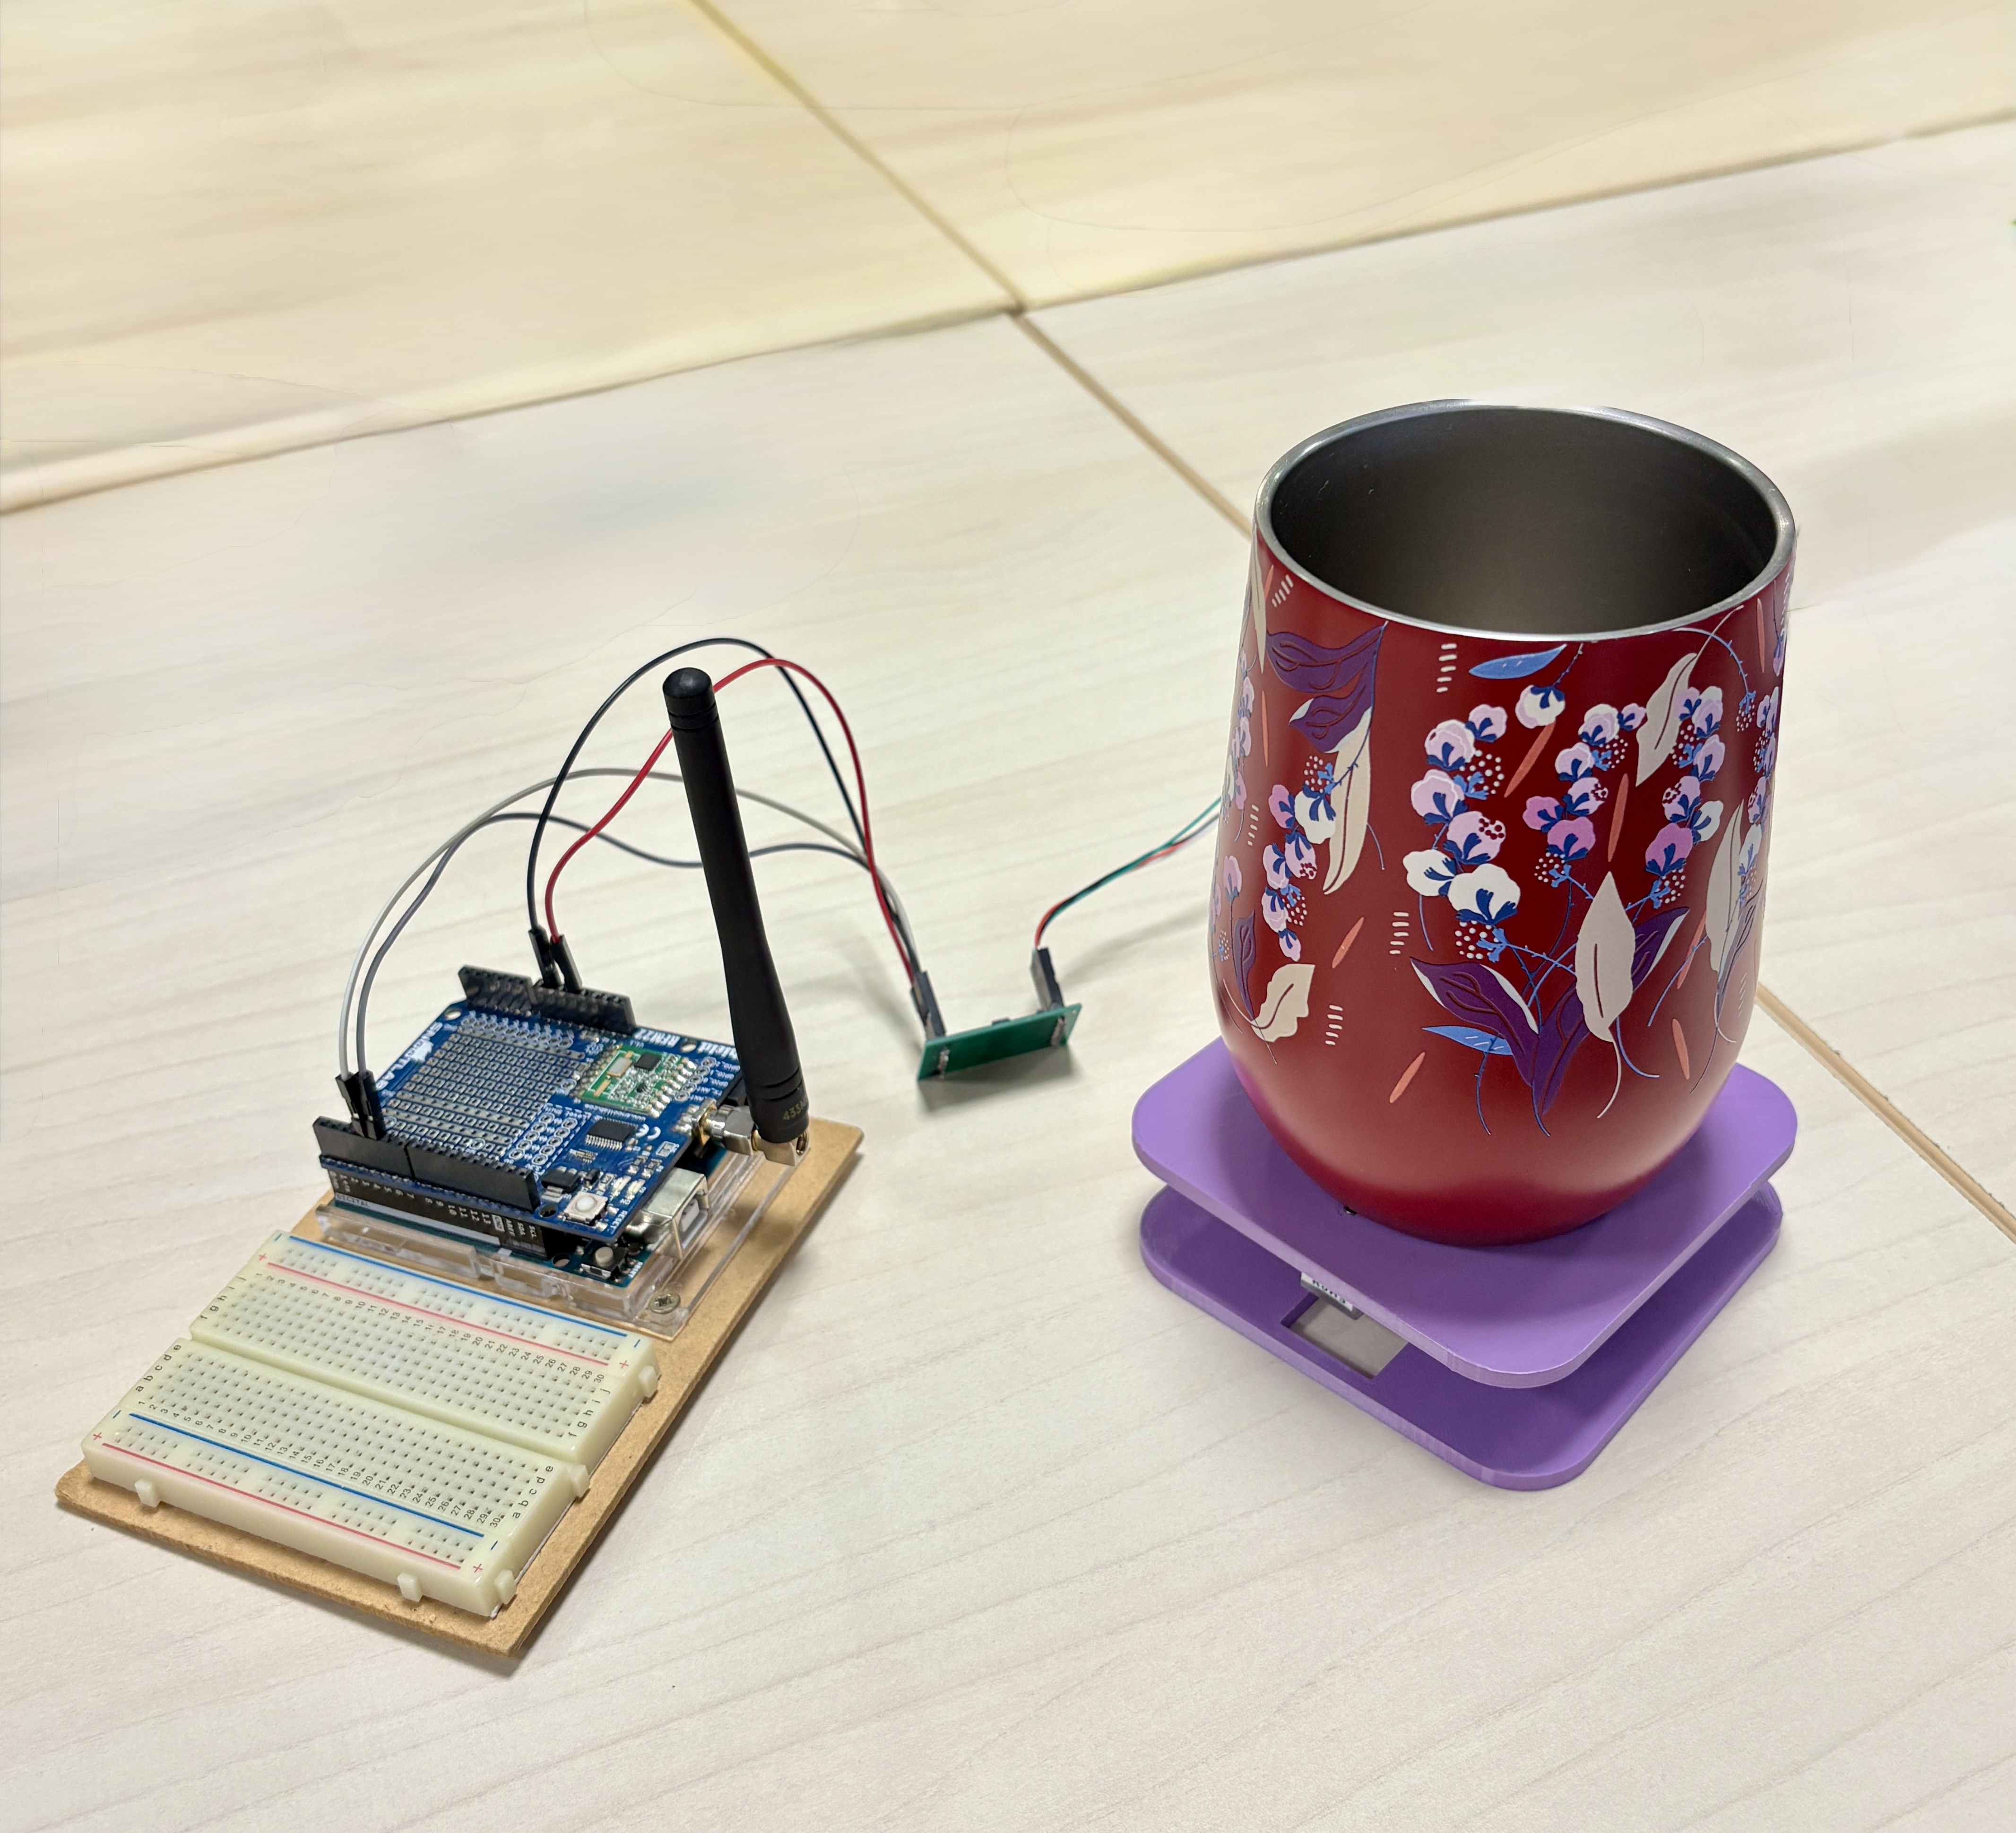
\includegraphics[width=\linewidth]{setup_images/set-up-with-cup.jpg}
        \caption{System setup with the cup placed on the coaster}
        \label{fig:setup-with-cup}
    \end{subfigure}
    \hfill
    \begin{subfigure}[b]{0.45\linewidth}
        \centering
        \includegraphics[width=\linewidth]{setup_images/set-up.jpg}
        \caption{System setup without the cup}
        \label{fig:setup-without-cup}
    \end{subfigure}
    \caption{Smart coaster hardware setup: with and without the cup}
    \label{fig:system-setup-views}
\end{figure}
